%---------------------- Problema 1 ------------------------------
\section*{Problema 1}


La barra de acero ($E = 206$ GPa y $S_y = 300$ MPa) en posici\'on vertical de la Figura ($L = 10$ m) tiene secci\'on transversal variable
\[
A(z) = A_0\, e^{-z/L}, \qquad A_0 = 1600\ \text{mm}^2,
\]
y est\'a sometida a una fuerza axial en su extremo libre ($P = 3$ kN). De acuerdo a la teor\'ia de barras, se pide:

\begin{enumerate}[label=\alph*), itemsep=4pt]
    \item Obtener la expresi\'on anal\'itica de los campos de tensi\'on y desplazamiento axial.
    \item Obtener la soluci\'on por MEF de dichos campos utilizando discretizaciones con 1, 2 y 4 elementos finitos de dos nodos de \'area constante en cada uno de ellos.
    \item Comparar y discutir las soluciones obtenidas en a) y b).
\end{enumerate}

\begin{center}
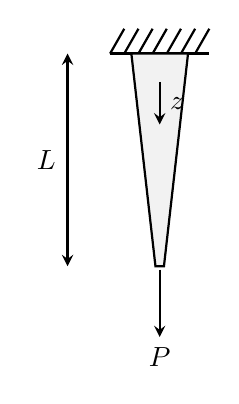
\begin{tikzpicture}[scale=0.9, >=stealth, thick]
    % apoyo empotrado (rayado)
    \draw[thick] (-0.7,3) -- (0.7,3);
    \foreach \x in {-0.7,-0.5,...,0.5}
        \draw (\x,3) -- (\x+0.2,3.35);

    % barra conica (mas ancha arriba, angosta abajo)
    \draw[thick, fill=black!5]
        (-0.4,3) -- (-0.06,0) -- (0.06,0) -- (0.4,3) -- cycle;

    % cota L
    \draw[<->] (-1.3,3) -- (-1.3,0);
    \node at (-1.6,1.5) {$L$};

    % eje z
    \draw[->] (0,2.6) -- (0,2.0);
    \node[right] at (0,2.3) {$z$};

    % carga P
    \draw[->] (0,-0.05) -- (0,-1.0);
    \node[below] at (0,-1.0) {$P$};
\end{tikzpicture}
\end{center}

\vspace{0.7cm}

%---------------------- Desarrollo -------------------------------

\begin{desarrollo}{a) Campos anal\'iticos de tensi\'on y desplazamiento}
    Para poder desarrollar esto lo que tenemos que hacer es un diagrama de la fuerza axial a la que cada parte de la barra se encuentra, para esto hacemos una funcion que la tenga en cuenta. Podemos tener en cuenta la fuerza axial de la barra en cada parte tenemos que saber si consideramos la fuerza peso o no, en caso que no lo contabilicemos se puede expresar asi la fuerza axial
    $$N(z)=3\text{k}N$$
    Con esto podemos calcular el esfuerzo axial
    $$\sigma_z(z)=\dfrac{N(z)}{A(z)}$$
    Una vez teniendo el esfuerzo podemos usar la propiedad constitutiba que relacion el esfuerzo con la deformacion, asumiento esfuerzo uniaxial, no hay efectos de adelgazamiento, tenemos 
    $$\sigma_z=E\varepsilon_z\longrightarrow \varepsilon_z=\dfrac{\sigma_z(z)}{E}=\dfrac{\partial w}{\partial z}$$
    
    $$\sigma_z(z)=\dfrac{3\text{k}N}{A_0e^{-z/L}}\quad \quad \varepsilon_z(z)=\dfrac{3\text{k}N}{EA_0e^{-z/L}}$$ 
    $$\dfrac{\partial w}{\partial z}=\dfrac{3\text{k}N}{EA_0e^{-z/L}}$$ 
    $$\int_{w_i}^{w_f} dw=\int_{\mathcal{B}}\dfrac{3\text{k}N}{EA_0e^{-z/L}}dz$$ 
    $$\delta_z=\dfrac{3000}{206\text{GPa}\cdot1600\text{mm}^2}\int_{\mathcal{B}}e^{z/L}dz$$
    $$\int_{0}^{L} e^{z/L} \, dz = \left[ L e^{z/L} \right]_{0}^{L}$$

$$\left[ L e^{z/L} \right]_{0}^{L} = L e^1 - L e^0 = L(e - 1)$$

$$\delta_z = \frac{3000 \text{N}\cdot 10\text{m}\cdot(e - 1)}{206000\text{MPa} \cdot 1600\text{mm}^2}$$
$$\delta_z \approx 0,1564\text{ mm}$$
\end{desarrollo}
\newpage
\begin{desarrollo}{b) Soluci\'on por MEF}
    \textit{Discretizaci\'on con 1 elemento}\\
    
    Para este caso nosotros tenemos este sistema
 \begin{center}
    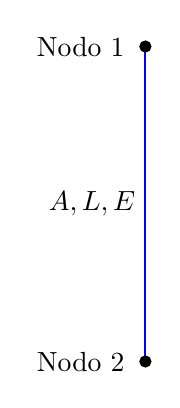
\begin{tikzpicture}
        % Dibujo de la barra
        \draw[thick, blue] (0,0) -- (0,-4)  node[midway, left, black] {$A,L, E$};
        
        % Nodo 1 (Superior)
        \filldraw[black] (0,0) circle (2pt) node[left=4pt] {Nodo 1};
        % Nodo 2 (Inferior)
        \filldraw[black] (0,-4) circle (2pt) node[left=4pt] {Nodo 2};
    \end{tikzpicture}
\end{center}
El cual se puede expresar como un resorte de constante $k=\dfrac{E}{AL}$
queda el balance de cada nodo como
\begin{align*}
    -k(u_2-u_1)&=R_1\\
    -k(u_1-u_2)&=F_1
\end{align*}
En forma matricial se veria asi
$$k\begin{bmatrix}
    1&-1\\
    -1&1
\end{bmatrix}\begin{bmatrix}
    u_1\\
    u_2
\end{bmatrix}=\begin{bmatrix}
    R_1\\
    F_1
\end{bmatrix}$$
Teniendo en cuenta las condiciones iniciales, tenemos que $u_1=0$ y $F_1=3\text{kN}$
Por ende la matriz de rigidez reducida como\\
$$F_1=u_2\cdot k\longrightarrow u_2=\dfrac{F_1}{k}$$
    \\
    \textit{Discretizaci\'on con 2 elementos}
    Para este caso nosotros tenemos este sistema
 \begin{center}
    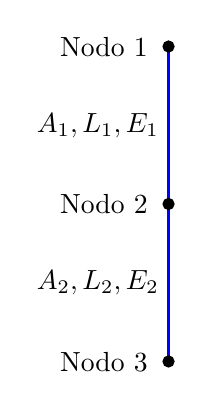
\begin{tikzpicture}
        % Dibujo de la barra
        \draw[thick, blue] (0,0) -- (0,-4);
        \node[left, black] at (0,-1){$A_1,L_1, E_1$};
        \node[left, black] at (0,-3){$A_2,L_2, E_2$};
        % Nodo 1 (Superior)
        \filldraw[black] (0,0) circle (2pt) node[left=4pt] {Nodo 1};
        % Nodo 2 (Inferior)
        \filldraw[black] (0,-2) circle (2pt) node[left=4pt] {Nodo 2};
        \filldraw[black] (0,-4) circle (2pt) node[left=4pt] {Nodo 3};
    \end{tikzpicture}
\end{center}
El cual se puede expresar como un resorte de constante $k=\dfrac{EA}{L}$
queda el balance de cada nodo como
\begin{align*}
    -k_1(u_2-u_1)&=R_1\\
    -k_1(u_1-u_2)-k_2(u_3-u_2)&=0\\
    -k_2(u_2-u_3)&=F_1
\end{align*}
En forma matricial se veria asi
$$\begin{bmatrix}
    k_1&-k_1&0\\
    -k_1&k_1+k_2&-k_2\\
    0&-k_2&k_2
\end{bmatrix}\begin{bmatrix}
    u_1\\
    u_2\\
    u_3
\end{bmatrix}=\begin{bmatrix}
    R_1\\
    0\\
    F_1
\end{bmatrix}$$
Teniendo en cuenta las condiciones iniciales, tenemos que $u_1=0$ y $F_1=3\text{kN}$
Por ende la matriz de rigidez reducida como\\




$$\begin{bmatrix}

k_1+k_2&-k_2\\
-k_2&k_2
\end{bmatrix}\begin{bmatrix}

    u_2\\
    u_3
\end{bmatrix}=\begin{bmatrix}

    0\\
    F_1
\end{bmatrix}$$

    \textit{Discretizaci\'on con 4 elementos}
    Para este caso nosotros tenemos este sistema
 \begin{center}
    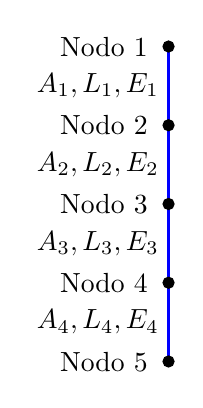
\begin{tikzpicture}
        % Dibujo de la barra
        \draw[thick, blue] (0,0) -- (0,-4);
        \node[left, black] at (0,-0.5){$A_1,L_1, E_1$};
        \node[left, black] at (0,-1.5){$A_2,L_2, E_2$};
        \node[left, black] at (0,-2.5){$A_3,L_3, E_3$};
        \node[left, black] at (0,-3.5){$A_4,L_4, E_4$};
        % Nodo 1 (Superior)
        \filldraw[black] (0,0) circle (2pt) node[left=4pt] {Nodo 1};
        % Nodo 2 (Inferior)
        \filldraw[black] (0,-1) circle (2pt) node[left=4pt] {Nodo 2};
        \filldraw[black] (0,-2) circle (2pt) node[left=4pt] {Nodo 3};
        \filldraw[black] (0,-3) circle (2pt) node[left=4pt] {Nodo 4};
        \filldraw[black] (0,-4) circle (2pt) node[left=4pt] {Nodo 5};
    \end{tikzpicture}
\end{center}
El cual se puede expresar como un resorte de constante $k=\dfrac{E}{AL}$
queda el balance de cada nodo como
\begin{align*}
    -k_1(u_2-u_1)&=R_1\\
    -k_1(u_1-u_2)-k_2(u_3-u_2)&=0\\
    -k_2(u_2-u_3)-k_3(u_4-u_3)&=0\\
    -k_3(u_3-u_4)-k_4(u_5-u_4)&=0\\
    -k_4(u_4-u_5)&=F_1
\end{align*}
En forma matricial se veria asi
$$\begin{bmatrix}
    k_1&-k_1&0&0&0\\
    -k_1&k_1+k_2&-k_2&0&0\\
    0&-k_2&k_2+k_3&-k_3&0\\
    0&0&- k_3&k_3+k_4&-k_4\\
    0&0&0&-k_4&k_4
    
\end{bmatrix}\begin{bmatrix}
    u_1\\
    u_2\\
    u_3\\
    u_4\\
    u_5
\end{bmatrix}=\begin{bmatrix}
    R_1\\
    0\\
    0\\
    0\\
    F_1
\end{bmatrix}$$
Teniendo en cuenta las condiciones iniciales, tenemos que $u_1=0$ y $F_1=3\text{kN}$
Por ende la matriz de rigidez reducida como\\

$$\begin{bmatrix}
    k_1+k_2&-k_2&0&0\\
    -k_2&k_2+k_3&-k_3&0\\
    0&-k_3&k_3+k_4&-k_4\\
    0&0&-k_4&k_4
    
\end{bmatrix}\begin{bmatrix}
    u_2\\
    u_3\\
    u_4\\
    u_5
\end{bmatrix}=\begin{bmatrix}
    0\\
    0\\
    0\\
    F_1
\end{bmatrix}$$
Ya ahora que ya tengo cada una de las matrices listas tengo que darle valor a cada una de $k_i$ para esto tengo el largo del elemento que no es muy difícil obtener ya que decidí hacerlos equidistantes uno con otro, pero esta el área que varia, para esto lo que aplico es el promedio entre el area inicial y el final del elemento\\

\textbf{1 elementos}
\begin{equation}
\mathbf{K} = \begin{bmatrix}
2.65e+04 & -2.65e+04 \\
-2.65e+04 & 2.65e+04 \\
\end{bmatrix}[\text{kN/m}]
\end{equation}
\textbf{2 elementos}
\begin{equation}
\mathbf{K} = \begin{bmatrix}
5.13e+04 & -5.13e+04 & 0 \\
-5.13e+04 & 8.25e+04 & -3.11e+04 \\
0 & -3.11e+04 & 3.11e+04 \\
\end{bmatrix}[\text{kN/m}]
\end{equation}
\textbf{4 elementos}
\begin{equation}
\mathbf{K} = \begin{bmatrix}
1.24e+05 & -1.24e+05 & 0 & 0 & 0 \\
-1.24e+05 & 2.34e+05 & -1.10e+05 & 0 & 0 \\
0 & -1.10e+05 & 2.06e+05 & -9.66e+04 & 0 \\
0 & 0 & -9.66e+04 & 1.82e+05 & -8.53e+04 \\
0 & 0 & 0 & -8.53e+04 & 8.53e+04 \\
\end{bmatrix}
\end{equation}

Para el caso de 1 elemento 

% ==========================================
% Vector de Desplazamientos Nodales [mm]
\begin{equation}
\mathbf{u} = \begin{bmatrix}
    0.00000 \\
    0.11331 \\
\end{bmatrix} \quad \text{[mm]}
\end{equation}

% ==========================================
% Tabla de Esfuerzos por Elemento [MPa]
\begin{center}
    
    \begin{tabular}{cccc}
        \hline
        \textbf{Elemento} & \textbf{Nodo 1} & \textbf{Nodo 2} & \textbf{Esfuerzo $\sigma$ [MPa]} \\
        \hline
        1 & 1 & 2 & 2.3342 \\
        \hline
    \end{tabular}
    \label{tab:esfuerzos 1}
\end{center}
Para el caso de 2 elementos (3 nodos)
% ==========================================
% Vector de Desplazamientos Nodales [mm]
\begin{equation}
\mathbf{u} = \begin{bmatrix}
    0.00000 \\
    0.05117 \\
    0.11687 \\
\end{bmatrix} \quad \text{[mm]}
\end{equation}

% ==========================================
% Tabla de Esfuerzos por Elemento [MPa]
\begin{center}

     \begin{tabular}{cccc}
        \hline
        \textbf{Elemento} & \textbf{Nodo 1} & \textbf{Nodo 2} & \textbf{Esfuerzo $\sigma$ [MPa]} \\
        \hline
        1 & 1 & 2 & 2.1082 \\
        2 & 2 & 3 & 2.7069 \\
        \hline
    \end{tabular}
    \label{tab:esfuerzos 2}
\end{center}

Para este caso tenemos 4 elementos, 5 nodos.
% ==========================================
% Vector de Desplazamientos Nodales [mm]
\begin{equation}
\mathbf{u} = \begin{bmatrix}
    0.00000 \\
    0.02418 \\
    0.05157 \\
    0.08261 \\
    0.11779 \\
\end{bmatrix} \quad \text{[mm]}
\end{equation}

% ==========================================
% Tabla de Esfuerzos por Elemento [MPa]
\begin{center}
    
    \centering
    \begin{tabular}{cccc}
        \hline
        \textbf{Elemento} & \textbf{Nodo 1} & \textbf{Nodo 2} & \textbf{Esfuerzo $\sigma$ [MPa]} \\
        \hline
        1 & 1 & 2 & 1.9920 \\
        2 & 2 & 3 & 2.2573 \\
        3 & 3 & 4 & 2.5578 \\
        4 & 4 & 5 & 2.8984 \\
        \hline
    \end{tabular}

    \label{tab:esfuerzos}
\end{center}

% ==========================================
% ==========================================

% ==========================================
\end{desarrollo}

\begin{desarrollo}{c) Comparaci\'on y discusi\'on}
Para esto lo que haremos sera graficar $\delta_z(z)$
\begin{center}
    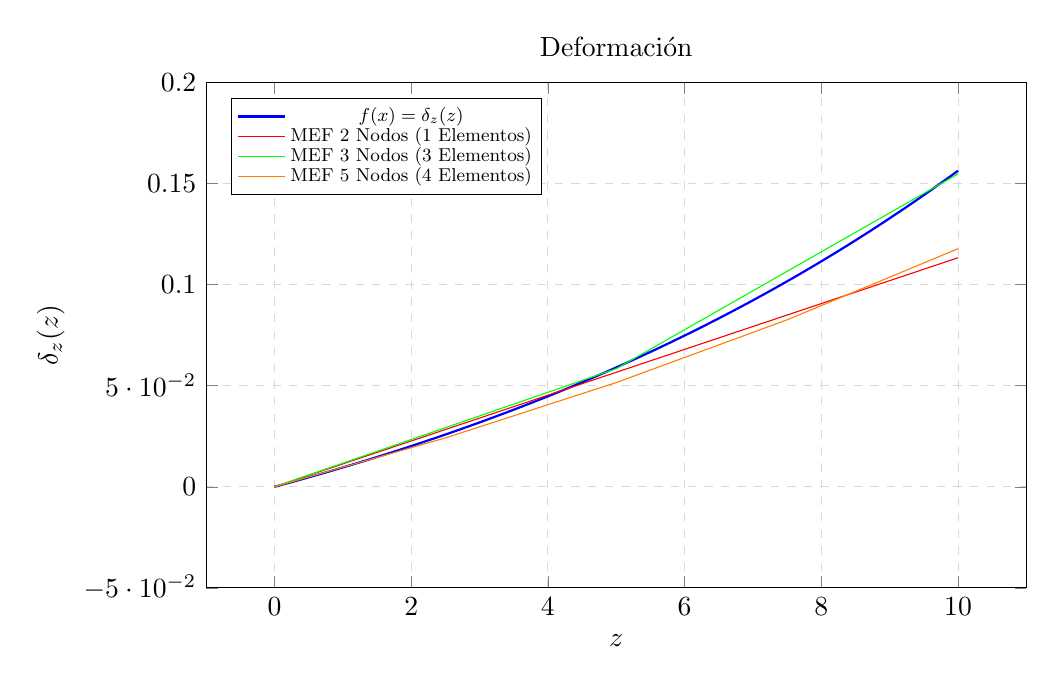
\begin{tikzpicture}
        \begin{axis}[
            title={Deformación},
            xlabel={$z$},
            ylabel={$\delta_z(z)$},
            grid=both, % Muestra la grilla
            grid style={dashed, gray!30},
            legend pos=north west, % Posición de la leyenda
            legend style={
    nodes={scale=0.75, transform shape}, % Escala todo el contenido al 75%
    font=\small,                         % Usa la fuente pequeña de LaTeX
    inner sep=2pt,                       % Reduce el relleno interior del recuadro
    row sep=-2pt                         % Junta un poco más las líneas de texto
},
            width=12cm,
            height=8cm,
            xmin=-1, xmax=11,
            ymin=-0.05, ymax=0.2
        ]
        
        % 1. Gráfica de la función continua
        \addplot [
            domain=0:10, 
            samples=100, % Cantidad de puntos para suavizar la curva
            color=blue,
            thick
        ]
        {3000*10000*(exp(x/10)-1)/(206000*1600)};
        \addlegendentry{$f(x) = \delta_z(z)$}
        

        
        \addplot [
            %%only marks, % Solo muestra los puntos, sin conectarlos con líneas
            mark=none, % Estilo del punto (círculo sólido)
            color=red,
            mark size=2.5pt
        ]
        coordinates {
    (0.0000, 0.00000)
    (10.0000, 0.11331)
};

        \addlegendentry{MEF 2 Nodos (1 Elementos)}
        
        \addplot [
            %%only marks, % Solo muestra los puntos, sin conectarlos con líneas
            mark=none, % Estilo del punto (círculo sólido)
            color=green,
            mark size=2.5pt
        ]
            coordinates {
        (0.0000, 0.00000)
        (5.0000, 0.05844)
        (10.0000, 0.15478)
    };

        \addlegendentry{MEF 3 Nodos (3 Elementos)}

        
        \addplot [
           % %only marks, % Solo muestra los puntos, sin conectarlos con líneas
            mark=none, % Estilo del punto (círculo sólido)
            color=orange,
            mark size=2.5pt
        ]
coordinates {
    (0.0000, 0.00000)
    (2.5000, 0.02418)
    (5.0000, 0.05157)
    (7.5000, 0.08261)
    (10.0000, 0.11779)
};


        \addlegendentry{MEF 5 Nodos (4 Elementos)}

                % 2. Gráfica del set de puntos (dispersión)
                % 2. Gráfica del set de puntos (dispersión)
%        \add¿plot [
            %%only marks, % Solo muestra los puntos, sin conectarlos con líneas
%            mark=none, % Estilo del punto (círculo sólido)
%            color=black,
%            mark size=2.5pt
%        ]
%        coordinates {
%    (0.0000, 0.00000)
%    (1.1111, 0.01069)
%    (2.2222, 0.02264)
%    (3.3333, 0.03599)
%    (4.4444, 0.05091)
%    (5.5556, 0.06758)
%    (6.6667, 0.08622)
%    (7.7778, 0.10704)
%    (8.8889, 0.13031)
%    (10.0000, 0.15632)
%};
%        \addlegendentry{MEF 10 Nodos}

        
        
        \end{axis}
    \end{tikzpicture}
\end{center}

Entonces ahora vamos a ver la diferencia de como se ven el ultimo nodos en todas las simulaciones MEF
\begin{center}  
    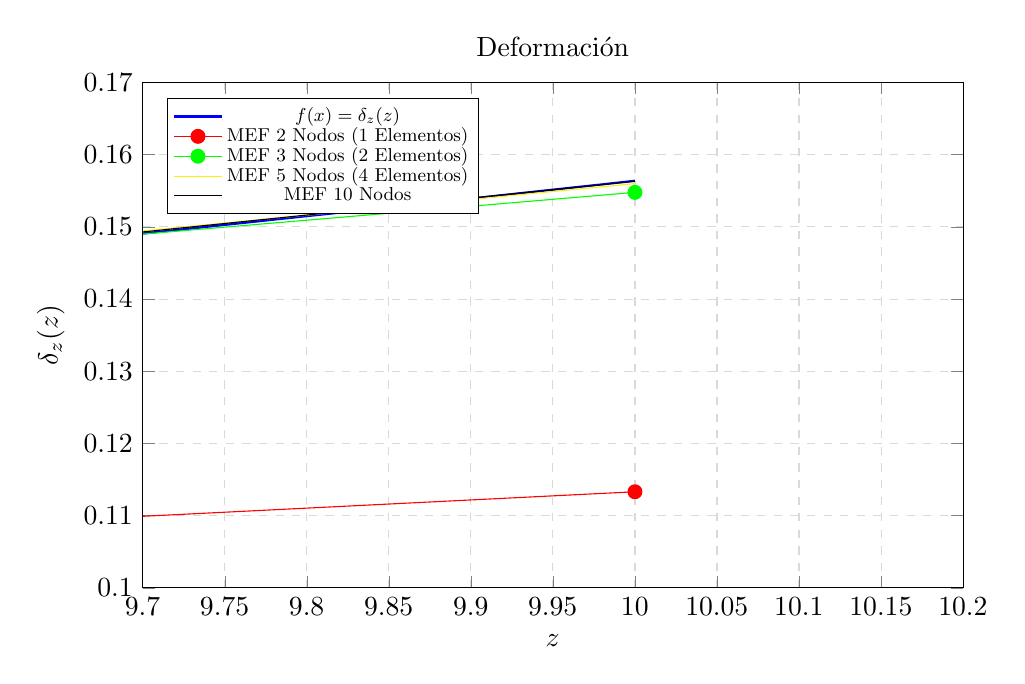
\begin{tikzpicture}
        \begin{axis}[
            title={Deformación},
            xlabel={$z$},
            ylabel={$\delta_z(z)$},
            grid=both, % Muestra la grilla
            grid style={dashed, gray!30},
            legend pos=north west, % Posición de la leyenda
            legend style={
    nodes={scale=0.75, transform shape}, % Escala todo el contenido al 75%
    font=\small,                         % Usa la fuente pequeña de LaTeX
    inner sep=2pt,                       % Reduce el relleno interior del recuadro
    row sep=-2pt                         % Junta un poco más las líneas de texto
},
            width=12cm,
            height=8cm,
            xmin=9.7, xmax=10.2,
            ymin=0.10, ymax=0.17
        ]
        
        % 1. Gráfica de la función continua
        \addplot [
            domain=9.5:10, 
            samples=100, % Cantidad de puntos para suavizar la curva
            color=blue,
            thick
        ]
        {3000*10000*(exp(x/10)-1)/(206000*1600)};
        \addlegendentry{$f(x) = \delta_z(z)$}
        

        
        \addplot [
            %only marks, % Solo muestra los puntos, sin conectarlos con líneas
            mark=*, % Estilo del punto (círculo sólido)
            color=red,
            mark size=2.5pt
        ]
        coordinates {
    (0.0000, 0.00000)
    (10.0000, 0.11331)
};
        \addlegendentry{MEF 2 Nodos (1 Elementos)}
        
        \addplot [
            %only marks, % Solo muestra los puntos, sin conectarlos con líneas
            mark=*, % Estilo del punto (círculo sólido)
            color=green,
            mark size=2.5pt
        ]
            coordinates {
        (0.0000, 0.00000)
        (5.0000, 0.05844)
        (10.0000, 0.15478)
    };

        \addlegendentry{MEF 3 Nodos (2
        Elementos)}

        
        \addplot [
            %only marks, % Solo muestra los puntos, sin conectarlos con líneas
            mark=none, % Estilo del punto (círculo sólido)
            color=yellow,
            mark size=2.5pt
        ]
            coordinates {
    (0.0000, 0.00000)
    (2.5000, 0.02578)
    (5.0000, 0.05889)
    (7.5000, 0.10140)
    (10.0000, 0.15599)
};


        \addlegendentry{MEF 5 Nodos (4 Elementos)}

                % 2. Gráfica del set de puntos (dispersión)
        \addplot [
            %only marks, % Solo muestra los puntos, sin conectarlos con líneas
            mark=none, % Estilo del punto (círculo sólido)
            color=black,
            mark size=2.5pt
        ]
        coordinates {
    (0.0000, 0.00000)
    (1.1111, 0.01069)
    (2.2222, 0.02264)
    (3.3333, 0.03599)
    (4.4444, 0.05091)
    (5.5556, 0.06758)
    (6.6667, 0.08622)
    (7.7778, 0.10704)
    (8.8889, 0.13031)
    (10.0000, 0.15632)
};
        \addlegendentry{MEF 10 Nodos}

        
        
        \end{axis}
    \end{tikzpicture}
\end{center}
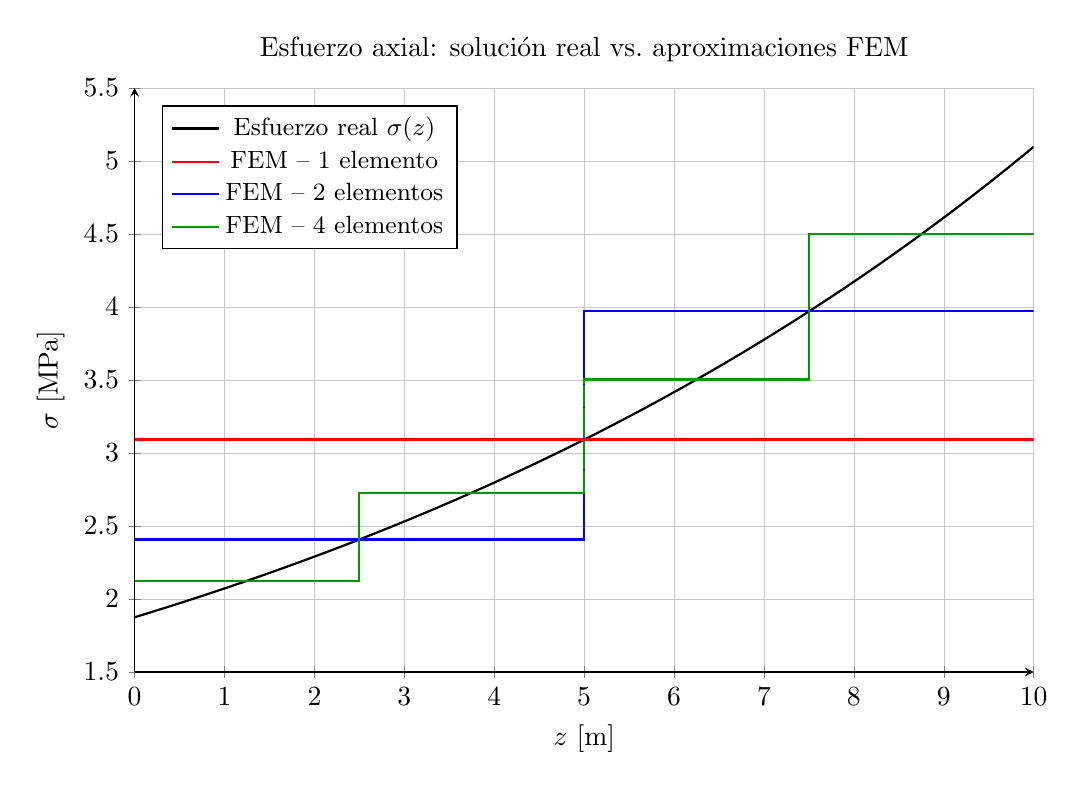
\begin{tikzpicture}
\begin{axis}[
    width=13cm, height=9cm,
    xlabel={$z$ [m]},
    ylabel={$\sigma$ [MPa]},
    title={Esfuerzo axial: solución real vs.\ aproximaciones FEM},
    xmin=0, xmax=10,
    ymin=1.5, ymax=5.5,
    grid=both,
    grid style={line width=.1pt, draw=gray!25},
    major grid style={line width=.2pt, draw=gray!45},
    legend pos=north west,
    legend style={font=\small},
    axis lines=left,
]
 
% --- Esfuerzo real (analitico): sigma(z) = 1.875 * exp(z/10) ---
\addplot[
    domain=0:10, samples=200,
    thick, black,
] {1.875*exp(x/10)};
\addlegendentry{Esfuerzo real $\sigma(z)$}
 
% --- 1 elemento (función escalón) ---
\addplot[
    const plot, thick, red, mark=none,
] coordinates {
    (0, 3.0914)
    (10, 3.0914)
};
\addlegendentry{FEM -- 1 elemento}
 
% --- 2 elementos (función escalón) ---
\addplot[
    const plot, thick, blue, mark=none,
] coordinates {
    (0, 2.4075)
    (5, 3.9694)
    (10, 3.9694)
};
\addlegendentry{FEM -- 2 elementos}
 
% --- 4 elementos (función escalón) ---
\addplot[
    const plot, thick, green!60!black, mark=none,
] coordinates {
    (0, 2.1247)
    (2.5, 2.7281)
    (5, 3.5030)
    (7.5, 4.4979)
    (10, 4.4979)
};
\addlegendentry{FEM -- 4 elementos}
 
% --- líneas punteadas verticales en los saltos (2 elementos) ---
\draw[blue, dotted, thick] (axis cs:5,2.4075) -- (axis cs:5,3.9694);
 
% --- líneas punteadas verticales en los saltos (4 elementos) ---
\draw[green!60!black, dotted, thick] (axis cs:2.5,2.1247) -- (axis cs:2.5,2.7281);
\draw[green!60!black, dotted, thick] (axis cs:5,2.7281)   -- (axis cs:5,3.5030);
\draw[green!60!black, dotted, thick] (axis cs:7.5,3.5030) -- (axis cs:7.5,4.4979);
 
\end{axis}
\end{tikzpicture}
Como podemos ver a medida que vamos aumentando la resolucion o la cantidad de nodos, de esta misma manera la cantidad de elementos el resultado se hace cada vez mas parecido al real
\end{desarrollo}

